%%%----------------------------------------------------------
\chapter{Texture Segmentation Using Laws Texture Energy Filters}
%%%----------------------------------------------------------

In this assignment the task was to perform a texture-based segmentation based on \textit{Laws texture energy maps}\cite{Laws1980}. A manually selected texture patch is used as reference texture. Since the calculation of Laws texture energy maps was already provided as an imageJ plugin it is not described in this assignment. The plugin creates 9 texture energy maps which were used to generate a 9-dimensional feature vector for every pixel. 

\section{Reference-base texture segmentation}

The goal is to segment the image into regions which have a similar texture as the reference texture:

\begin{enumerate}
	\item Select a region of interest $R$.
	\item Create the 9 texture energy maps with the help of the plugin.
	\item Calculate the reference feature vector $x_R$ for the region of interest.
	\item Create a distance map which holds the distance between the local feature vector and the reference feature vector.
	\item Apply automatic thresholding to the distance map to obtain the final segmentation.
\end{enumerate}

\subsection{Calculate the reference feature vector}
To create the reference feature vector $x_R$ sum up all the local feature vector values of each pixel $x_k(u,v)$ in the marked region of interest and divide each value by the number of pixels in the region $|R|$ as stated in the following equation:
\begin{equation}
	x_R = \frac{1}{|R|} \cdot \sum_{(u,v)\in R} x(u, v)
\end{equation}

This results in the 9-dimensional reference feature vector.

\subsection{Calculate the distance map}
To setup a distance map $D$ the distance between the local feature vector $x(u,v)$ and the reference feature vector $x_R$ needs to be calculated:
\begin{equation}
	D(u,v) = ||x(u,v) - x_R||
\end{equation}

The L1 as well as the L2 distance norm were used.

After the distance map is created automatic Otsu thresholding was applied to the distance map $D$ to obtain the final segmentation.

\subsection{Result}

Figure \ref{fig:TestImage1}, \ref{fig:TestImage2} and \ref{fig:TestImage3} show the results of some test images. The results show the original image on the left then the distance map and the distance map after thresholding on the right. In most cases the segmentation worked quite well.
Overall the L2 distance norm showed better results. In some cases by quite a bit as shown in Figure \ref{fig:DistanceNorm}.

\begin{figure}
	\centering
	\begin{minipage}[t]{0.49\linewidth}
		\centering
		\frame{
\includegraphics[width=.95\linewidth]{images/ass07image02l1}}
	\end{minipage}
	\hfill
	\begin{minipage}[t]{0.49\linewidth}
		\centering
		\frame{
\includegraphics[width=.95\linewidth]{images/ass07image02thresh}}
	\end{minipage}
	\caption{Texture Segmentation. Using the L1 norm on the left side and the L2 norm on the right.}
	\label{fig:DistanceNorm}
\end{figure}

\begin{figure}
	\centering
	\begin{minipage}[t]{0.32\linewidth}
		\centering
		\frame{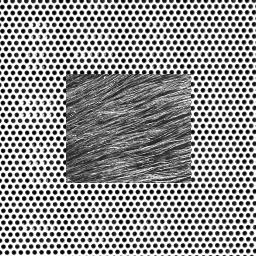
\includegraphics[width=.95\linewidth]{images/ass07image01origin}}
	\end{minipage}
	\hfill
	\begin{minipage}[t]{0.32\linewidth}
		\centering
		\frame{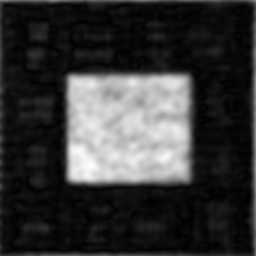
\includegraphics[width=.95\linewidth]{images/ass07image01distance}}
	\end{minipage}
	\begin{minipage}[t]{0.32\linewidth}
		\centering
		\frame{
\includegraphics[width=.95\linewidth]{images/ass07image01thresh}}
	\end{minipage}
	\caption{The outer texture was selected as reference texture. Image size: 256 x 256.}
	\label{fig:TestImage1}
\end{figure}

\begin{figure}
	\centering
	\begin{minipage}[t]{0.32\linewidth}
		\centering
		\frame{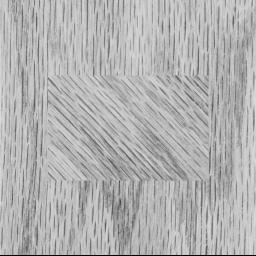
\includegraphics[width=.95\linewidth]{images/ass07image02origin}}
	\end{minipage}
	\hfill
	\begin{minipage}[t]{0.32\linewidth}
		\centering
		\frame{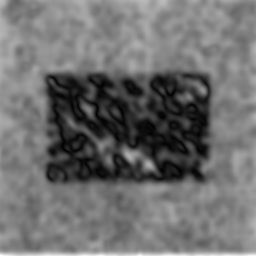
\includegraphics[width=.95\linewidth]{images/ass07image02distance}}
	\end{minipage}
	\begin{minipage}[t]{0.32\linewidth}
		\centering
		\frame{
\includegraphics[width=.95\linewidth]{images/ass07image02thresh}}
	\end{minipage}
	\caption{The inner texture was selected as reference texture. Image size: 256 x 256.}
	\label{fig:TestImage2}
\end{figure}

\begin{figure}
	\centering
	\begin{minipage}[t]{0.32\linewidth}
		\centering
		\frame{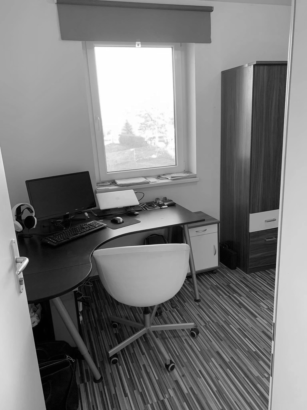
\includegraphics[width=.95\linewidth]{images/ass07image03origin}}
	\end{minipage}
	\hfill
	\begin{minipage}[t]{0.32\linewidth}
		\centering
		\frame{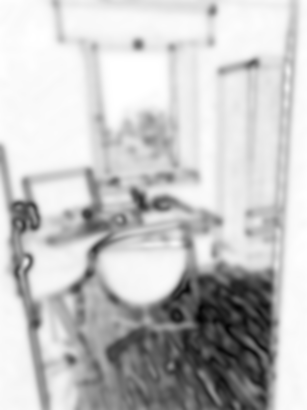
\includegraphics[width=.95\linewidth]{images/ass07image03distance}}
	\end{minipage}
	\begin{minipage}[t]{0.32\linewidth}
		\centering
		\frame{
\includegraphics[width=.95\linewidth]{images/ass07image03thresh}}
	\end{minipage}
	\caption{The floor was selected as reference texture. Image size: 307 x 410.}
	\label{fig:TestImage3}
\end{figure}
